\documentclass[a4paper,english]{report}
\usepackage[latin1]{inputenc}
\usepackage{babel}
\usepackage[margin=2.5cm,nohead]{geometry}
\usepackage{graphicx}
\usepackage{color}
\bibliographystyle{plain}
\setlength{\parskip}{1.5ex}
\sloppy

\begin{document}
\title{Blue Flash Memory Technology}

\author{
Ant�nio Augusto Fr�hlich\\
Marcelo Trierveiler Pereira\\
Arliones Stevert Hoeller Junior\\
Felipe Zimmermann Homma
}

\maketitle

%%%%%%%%%%%%%%%%%%%%%%%%%%%%%%%%%%%%%%%%%%%%%%%%%%%%%%%%%%%%%%%%%%%%%%%%
\chapter{Flash Memory Technology}

This chapter brings an overview of Flash Memory Technologies, aiming at
establishing the state-of-the-art in the field and serving as a basis
for the forthcoming sections of this text.

Flash memory is a solid-state, non-volatile, re-writable memory that
works like a \emph{Random Access Memory} [RAM] unit and a hard disk
drive combined. Flash memory stores bits of electronic data in memory
cells, just like DRAM, but it also works like a hard-disk drive in that
when the power is turned off, the data remains in memory. Because of its
high speed, durability, and low voltage requirements, flash memory is
ideal for use in many applications, such as digital cameras, cell
phones, printers, handheld computers, pagers, and audio
recorders~\cite{Grossman:1996}.


\section{General Concepts}

\emph{Flash Memories} are very similar to \emph{Electrically Erasable
  Programmable Read-Only Memories} [EEPROM], the main difference being
that flash memories can only be erased in chunks (called sectors), and
this is the origin of its name (erase sectors in a ``flash'').  Such
erasing scheme simplifies the circuitry, allowing for a greater density
in regard to an equivalent EEPROM. Actually, flash memories can achieve
densities similar to EPROMs. 

There are several technologies a flash memory cell can be built on: NOR,
DINOR, T-Poly, AND, NAND; each of which requires a particular
programming and erasing method~\cite{st-flash:2001}. These technologies
allow flash memories to retain stored data without a permanent power
supply for periods as long as twenty years. Nevertheless, the very same
technologies are responsible for one of the biggest shortcomings of
flash memories: the limitation in the number of write/erase operations
that can be performed before material fatigue becomes critical and
compromises data consistency. Notwithstanding, the typical rewrite limit
(in the order of hundred thousands) is acceptable for many applications.

Since flash memories can only be erased in sectors, the size of a sector
becomes a crucial operational factor for such memories. In order to
allow for a more rational use of the memory available in a flash, some
models provide sectors of different sizes and properties. For instance,
a smaller ``boot sector'' can be provided that supports
write-protection, or yet an special sector can hold a unique serial
number assigned at manufacturing-time.


\section{Architectural Overview}

Flash, EPROM, and EEPROM devices use basically the same floating gate
mechanism to store data, but they deploy distinct reading and writing
mechanisms~\cite{Katti:1994}. In all cases, the basic memory cell
consists of a single \emph{MOS transistor} [MOSFET] with two gates: a
\emph{control gate} that is connected to the read/write control
circuitry and a \emph{floating gate} that is located between the control
gate and the channel --- the part of the MOSFET through which an
electric current can flow between the so-called \emph{source} and
\emph{drain} terminals.

\begin{figure}[h]
\centering
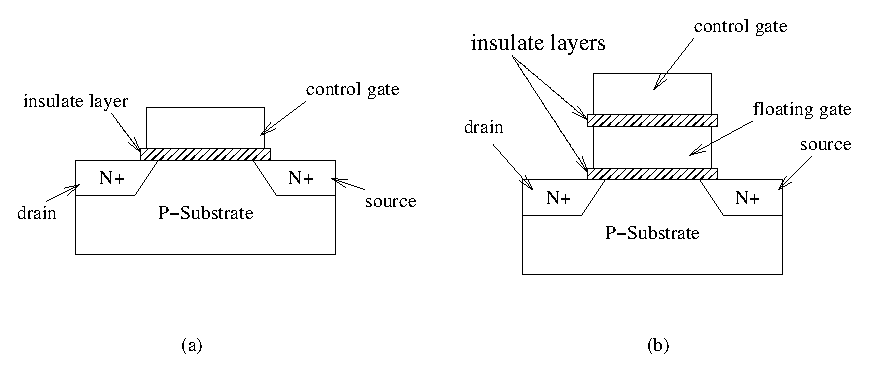
\includegraphics{MOSFETandFGT}
\caption{schematic of (a) MOSFET and (b) floating-gate transistor.\label{fig:MOSFETandFGT}}
\end{figure} 

In a standard MOSFET, a single \emph{gate} terminal controls the
electrical resistance of the channel: an electric voltage applied to the
\emph{gate} controls how much current flows between \emph{source} and
\emph{drain}.  Figure~\ref{fig:MOSFETBehaviour} illustrates the behavior
of such a kind of transistor.  Current is only present in the channel if
a voltage is applied to the control gate. The voltage needed to build up
the ``bridge'' over the channel is commonly called \emph{Threshold
  Voltage} (Vt). The MOSFETs used in non-volatile memories include a
\emph{second gate} that is completely surrounded by an insulating layer,
that is, it is electrically insulated from the rest of the circuitry
(see figure~\ref{fig:MOSFETandFGT}).

\begin{figure}[h]
\centering
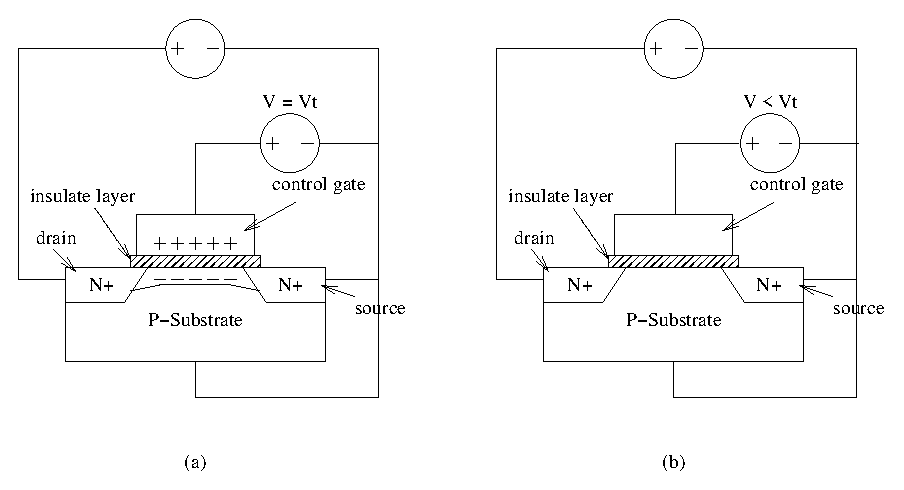
\includegraphics{MOSFETBehaviour}
\caption{MOSFET behavior: with (a) and without (b) current. 
  \label{fig:MOSFETBehaviour}}
\end{figure} 

Because the floating gate is physically very close to the MOSFET
channel, even a small electric charge has an easily detectable effect on
the electrical behavior of the transistor. By applying appropriate
signals to the control gate and measuring the change in the transistor
behavior, it is therefore possible to determine whether or not there is
an electric charge on the floating gate (see figure~\ref{fig:FGTBehav}).
In a floating-gate transistor, Vt will be linked with the number of
electrons trapped in the floating-gate.  It will be as high as the
number of electrons trapped in the floating-gate.  Similarly to a
MOSFET, the flow in the channel is from source to drain.


\begin{figure}[h]
  \centering 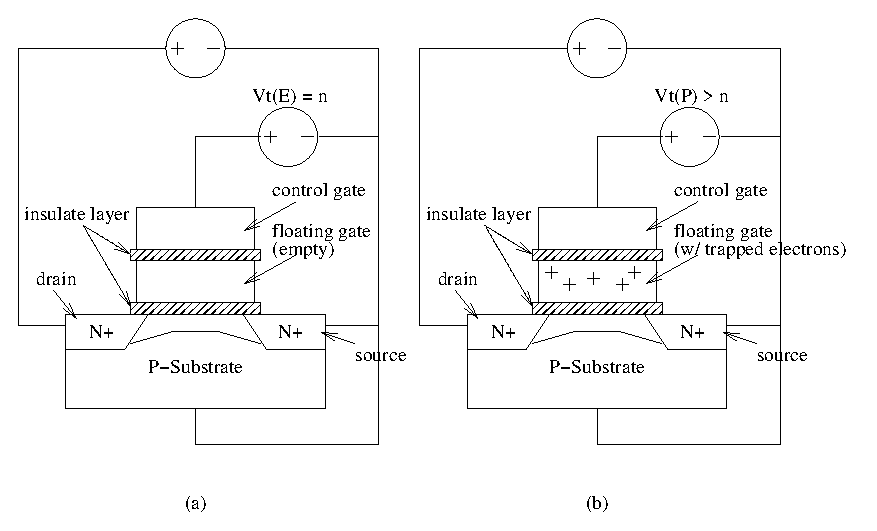
\includegraphics{FGTBehaviour}
\caption{Floating-gate transistor behavior: (a) without and (b) with
trapped electrons.\label{fig:FGTBehav}}
\end{figure} 

Since the floating gate is electrically insulated from the rest of the
transistor, special techniques are required to move electrons to and
from it. One technique consists in filling the MOSFET channel with
high-energy electrons by applying relatively high voltages to the
control gate and the drain of the MOSFET. Some of these "hot" electrons
have sufficient energy to cross the barrier between the channel and the
floating gate. When the high voltages are removed, these electrons
remain trapped on the floating gate. This is the method used to program
a memory cell in EPROM and flash memories.

This technique, known as \emph{Channel Hot Electron} [CHE] injection,
can be used to load an electric charge onto the floating gate, but does
not provide a way to discharge it.  In order to discharge a floating
gate, flash memories\footnote{In EPROM memories, the floating gate is
  discharged by flooding the entire memory array with ultra-violet light
  --- the high-energy light penetrates the chip structure and impart
  enough energy to the trapped electrons, allowing them to escape the
  floating gate.}  tackle on a quantum effect known as \emph{tunneling}:
electrons are removed from the floating gate by applying a voltage to
the MOSFET that is large enough to cause electrons to 'tunnel' across
the insulating layer~\cite{Rajkanan:1996}.

Traditionally, the floating gate mechanism has been used to store a
single data bit, which is read by comparing the MOSFET threshold voltage
with a reference value.  More sophisticated techniques make it possible
to distinguish more than two floating gate charge states, thus enabling
two or more bits to be stored on a single floating gate. This is an
important technology breakthrough, because storing two bits/cell doubles
the memory capacity for a given cell size~\cite{intel-flash:2002}.


\section{Operation}

There are three basic operations that can be performed on a flash:
\emph{read}, \emph{program}, and \emph{erase}. Reading and programming a
flash is usually as fast as the equivalent operations on a DRAM (read
and write), but the erasing operation is much slower than reading or
programming.  This shortcoming is being tackled through partitioning and
also through the inclusion of pause operations that allow for operating
interweaving in a single partition.

The execution of these operations is managed and validated by the flash
own state-machine. Usually, the state-machine of a flash is also able to
detect operation time-outs, which may be an indicative of cell
degeneration.

\paragraph{Reading:}

reading from a flash memory is similar to reading from traditional
memory devices (e.g. DRAM). In order to reduce latency and improve
bandwidth, some flash memory units deploy sophisticate access modes:
besides traditional asynchronous bit and word read modes, they often
support asynchronous page read (buffering a whole page to speedup
subsequent accesses to the same page) and synchronous burst read
(multiple data words from a single address).

Figure~\ref{fig:ReadingFGT} illustrates the procedure of reading a flash
cell. Applying a reading voltage (Vt(R)) to the control gate can produce
one of two situations: (a) if the floating-gate is empty, current will
be detected in the channel; or (b) if there are electrons in the
floating-gate, then no current will formed. It is also possible to
define several levels for Vt by controlling the number of electrons in
the floating-gate. This is the principle of multilevel cells, which rely
on different states to store more than a bit per transistor.

\begin{figure}[h]
\centering
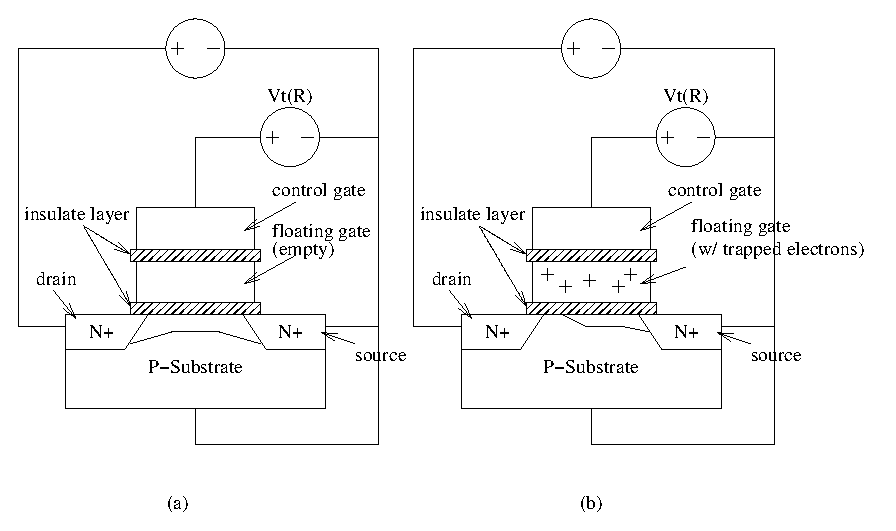
\includegraphics{ReadingAFGT}
\caption{Reading operation on a floating-gate transistor.\label{fig:ReadingFGT}}
\end{figure} 

\paragraph{Programming:}

a typical flash memory is delivered with all sectors erased, i.e. with
all bits set to ``1''. Thus, programming (writing to) a flash consists
in turning some ``1s'' into ``0s''. Note that the reverse operation,
turning ``0s'' into ``1s'', is not defined\footnote{Trying to program a
  previously zeroed bit of a flash to ``1'' usually has no effect,
  though it probably causes the flash's state-machine to signalize a
  condition flag that might trigger external events.}. The only way to
set a bit in a flash is by erasing the whole sector. Some flash models
support programming single bits, words, and even blocks (burst write).
Some models also provide buffers to speed up programming, thus
supporting a write operating similar to DRAM (as long as one does not
try to overwrite a ``0'' with an ``1''). At transistor level, programming
a flash consists in injecting electrons into the floating gate.

\paragraph{Erasing:}

Erasing a sector of a flash memory unit, i.e. setting all of its bits to
``1'', is achieved by removing electrons from floating gates. Depending
on the technology used, a flash memory may be subjected to the so called
``over-erasing'' phenomenon: erasing a cell whose value is already ``1''
puts that cell in a state that prevents further programming. Flashes
exposed to the phenomenon usually handle it internally by programming
all bits of a sector (setting to ``0'') before erasing them (setting to
``1''). Therefore, erasing a flash becomes a trivial operation for
firmware/driver programmers.


\textcolor{black}{
\section{On the Market}
}

\textcolor{black}{
Since the invention of the flash memory, manufacturers have been looking
for alternatives to increase performance and capacity. As flash memories
gain new markets, technologies are being incorporated to turn it a more
reliable choice over other persistent memory technologies. Some of the
most significant improvements now available on the market are:
}

\begin{description}
\item[Non-Uniform Sector Size Architecture:] some models are designed
  with non-uniform sector size. They allow for specialized sectors such
  as boot sectors and sensitive date without waste of space.
  
\item[Common Flash Interface \protect{[CFI]}:] specifies a standard
  command set for flash memories. It has been pushed by market leaders
  in an attempt to make the development of flash software vendor
  independent.
  
\item[Multi-partitions Architecture:] multi-partition or multi-bank
  architecture supports multiple operations to be simultaneously
  performed on the same flash memory unit, thus allowing for parallel
  operation.
  
\item[Multilevel Cell Technology:] multilevel cell intends to raise the
  density (i.e. amount of bits) of the flash without raising the dye
  area. This is reached by controlling the amount of electrons that are
  trapped in the floating-gate as discussed earlier in this section.
  Typical models of multilevel cell flash memories store 2 bits per
  cell. 
  
\item[Security:] some models include security registers ---one-time
  programming sectors or sectors dedicated to store security data (like
  unique identifier numbers).

\end{description}


\textcolor{blue}{
\subsection{Case Studies}
}

\textcolor{blue}{
The forthcoming discussion presents several flash memory technologies
currently available on the market. The purpose of this section is
to identify each technology highlights.
}

\textcolor{blue}{
\subsubsection{AMD}
}

\textcolor{blue}{
http://www.amd.com/
}

\textcolor{blue}{
AMD delivers various CFI compliant models, with operational voltages
ranging from 1.8V to 5.0V, densities up to 256 Mb and with boot sectos
(top or bottom configurations). Their products operate in temperatures
from commercial (0 --- $+70^o$ C) to super-extended (-55 --- $+145^o$
C).
}

\textcolor{blue}{
They have models with multi-partitions, MirrorBit technology and Dual
Operation (Flash + SRAM hybrid). For safety reasons, their products
are able to lock one dedicated sector.
}

\textcolor{blue}{
\paragraph{Dual Operation:} by incorporating a SRAM unit AMD delivers 
a ``hibrid'' flash model that can make multiple operations without
partitioning the memory. All operations are executed on the SRAM unit
and later committed to flash.
}

\textcolor{blue}{
\paragraph{MirrorBit Technology:} AMD multi-bit technology. This technology 
differs from the other manufacturers by implementing two distinct bits
instead of $2^{2}$ states to create two bits. This way they can offer
a high density model without compromising performance or
reliability. This is done by building a symmetrical transistor with
the sources and drain replicated in both sides (see Figure
\ref{fig:MirrorBitschematic}), and with a very careful and controled
injection of electrons in one side of the floating gate.
}

\begin{figure}[h]
\centering 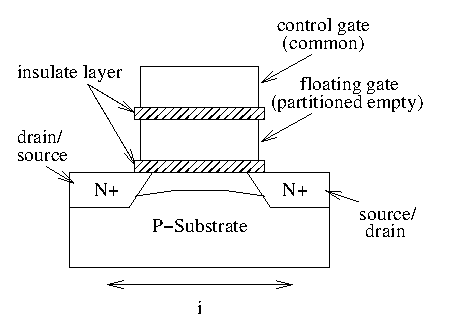
\includegraphics{MirrorBit}
\caption{MirrorBit transistor schematic.\label{fig:MirrorBitschematic}}
\end{figure}

\textcolor{blue}{
\subsubsection{Intel}
}

\textcolor{blue}{
http://www.intel.com/
}

\textcolor{blue}{
Intel products operates in voltages from 1.8 V to 5 V, some models have
higher output voltages for compatibility purposes; they have
multi-partition, non-uniform size sectors (boot sectors in top or
bottom configuration) and multilevel cell technology (StrataFlash
models), all CFI compliant.
}

\textcolor{blue}{
Security mechanism is a bunch of bits composed by two parts: 
one programmed by Intel and other programmed by the user.
}

\textcolor{blue}{
Besides the BCS, Intel have the Extended Command Set (ECS) CFI
compliant, which makes use of their own hardware character.
}

\textcolor{blue}{
\paragraph{Enhanced Factory Programming (EFP) and Buffered Enhanced Factory Programming (BEFP):} these 
two Intel exclusive technologies are used to minimize the flash
programming in controlled environments, usually to pre-program the
chip and put it in the equipment later. This is made by turning all
data checks off during the program stage, verifying all the
correctness later. Both technologies are the same, but one applies to
standard flash memories and other to Strata (multilevel) flash
memories.
}

\textcolor{blue}{
\subsubsection{ST Semiconductors}
}

\textcolor{blue}{
http://us.st.com/
}

\textcolor{blue}{
ST have multi-level cell technology, multi-partitions, boot sector (top
or bottom configurations), programmable security sector and CFI
compliance. Voltages from 1.8 to 5.0V, temperatures from commercial to
super-extended.
}

\textcolor{blue}{
ST Semiconductors has a range of specialized products to the automotive market. Their
M29F (5V) and M29W (3V) families can operate in automotive environment
( -$40^o$ to +$125^o$ C); M58BF008 (8Mb) and M58BW016 (16Mb) models are
dedicated to this application class.
}

\textcolor{blue}{
\subsubsection{ATMEL}
}

\textcolor{blue}{
http://www.atmel.com/
}

\textcolor{blue}{
ATMEL flash memories operate in voltages from 2.7 to 5V, 512 to 32
Mbits densities, concurrent Read \& Write, boot sector,
multi-partitions and frequencies reaching 100 MHz. In some models it
is possible to define 16 or 32 bits databus.
}

\textcolor{blue}{
\paragraph{Fast Programming Time:} if there is high voltage available (12V), it is possible to reach very
high programming speeds (30us per word/double word).
}

\textcolor{blue}{
\paragraph{Serial Flash:} serial flash memory uses Serial Peripheral Interface (SPI), and it can
be used as replacement for SPI compliant EEPROMs, without changes of
the board layout (if pinage also compatible). It operates at 20 MHz
and in low voltages (2.7---3.6 V), densities ranging from 512 Kbits to
over 4 Mbits.
}

\textcolor{blue}{
\paragraph{Data Flash:} SPI compliant hybrid serial/parallel flash memory.
}

\textcolor{blue}{
\subsubsection{MICRON}
}

\textcolor{blue}{
http://www.micron.com/
}

\textcolor{blue}{
Micron products are CFI compliant and have their own extensions
(SCS). Their products have dedicated boot sector (in top or bottom
configuration), multi-partition architecture, operational voltages
from 2.7 to 5.0V, select databus size (8 or 16 bits), temperatures
varying from commercial to extended.
}

\textcolor{blue}{
\paragraph{SynchFlash:} this family, a SDRAM similar interface (that can imitate a SDRAM chip)
is introduced. It has high read performance (equals SDRAM read
performance) consequently turned the chip into a very competitive
choice for execute-in-place applications. This Family is second
sourced by ATMEL. There are plans (in a near future) to reach the same
read performance of DDR SDRAM.
}

\textcolor{blue}{
\section{Future of Non-volatile Memory Technologies}
}

\textcolor{blue}{
Today flash memory is the best choice for fast and small persistent
storage due to its high speed and density, but new technologies are
coming, specially those utilizing magnetic media. There are also other
researches in optics and nanotechnology areas.
}

\textcolor{blue}{
The new material and new research tools, make the creation of new
storage medias and devices possible. The near future promises faster
and more dense devices than flash memory.
}

\textcolor{blue}{
By now ferroelectric and magneto-resistive memory have great potential
to be deployed with great advantage over flash memory, because these
technologies are not based on read-only schema. For future of
holographic devices, we can expect a massive storage at great
speeds. IBM has been studying nanotechnology since
1990 and the prototypes are promissing.
}

\textcolor{blue}{
\subsection{Future of Flash}
}

\textcolor{blue}{
Flash memory will be faster and more dense and reliable. Read speed
increases are visible even these days, by buffering, paging and other
indirect access techniques. But flash devices will be limited by
integrated circuit technology and material limits.
}

\textcolor{blue}{
Advanced manufacturing techniques can reduce the size of the tracks
and transistors giving flash memory more density, raising the write
speed, but its scale limits are bound to material (silicon) limits.
}

\textcolor{blue}{
Unfortunately this technology was based on read-only memory technology
and thus, writing will continue to be the bottleneck, and maybe the
hybrid systems (embedded RAM + Flash) will partially manage this
issue.
}

\textcolor{blue}{
\subsection{Holography}
}

\textcolor{blue}{
Holography was first proposed as a data storage technology in the
early 1960's, by a Polaroid scientist named Pieter J. van Heerden
\cite{Heerden:1963}. Ten years later, RCA Laboratory's scientists
recorded 500 holograms in a specially made crystal, and 550 holograms
in a light sensitive polymer material \cite{Stewart:1973}. Even with
those great results, due to the absence of cheap and appropriate
components and the crescent successful researches on magnetic and
semiconductor memories, the development of holographic data storage
artifacts was placed on hold.
}

\textcolor{blue}{
Nevertheless, the recent advent of appropriate components (such as
more powerful laser diodes) and the low prices achieved by the needed
material, finally yielded the retake of holographic data storage
researches \cite{AshleyETAL:2000}.
}

\textcolor{blue}{
The latest published materials state that, with the current
technologies, it is possible to develop an holographic storage system
with a bandwidth of tens of~GB/s, which is the optical limit. The
problem with this system is its recording rate (only a few tens
of~KB/s). Nevertheless, the scientists say that future technologies
might improve this value up to one~GB/s~\cite{CLDP:1999}.
}

\textcolor{blue}{
Another interesting characteristic of holographic data storage systems
is its density. Theoretically it could reach a density of tens of~$\rm
Tb/cm^3$, but, there is no such precise technologies yet to allow this
density. Recent experiments can only record some tens of~$\rm
Mb/cm^3$, but some researchers say they would reach a density of one
or two~$\rm Gb/cm^3$ in a short time, which can lower its cost
\cite{CLDP:1999}.
}

\textcolor{blue}{
An example of a Holographic System is showed in
Figure~\ref{fig:HolographicSample}. The SLM (Spatial Light Modulator)
contains the data that will be recorded. This processes is done by the
interference generated by the laser beam that illuminates de SLM and
the called reference laser beam, which cames from the Reference
Array. To read data, only the Laser beam illuminates the fully opened
SLM, and the image of the wanted page is projected on the Detector.
}

\begin{figure}[h]
\centering
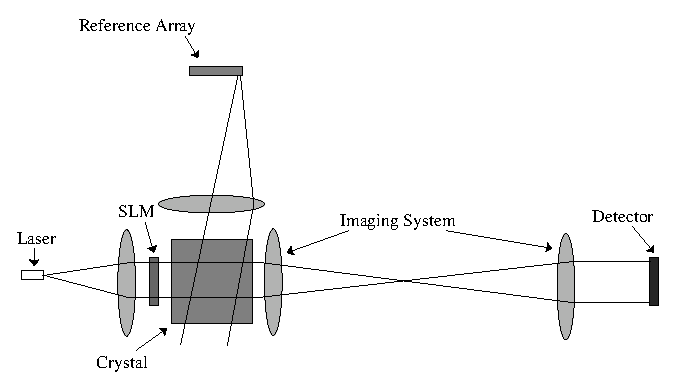
\includegraphics{Holography}
\caption{An example of holographic system.
\label{fig:HolographicSample}}
\end{figure}

\textcolor{blue}{
The are many multinational companies that have research teams working
on Holography, some of those are IBM~\cite{IBM:2003},
Lucent~\cite{Lucent:2003}, Kodak~\cite{Kodak:2003},
Imation~\cite{Imation:2003}, Panasonic~\cite{Panasonic:2003},
Sony~\cite{Sony:2003} and NEC~\cite{NEC:2003}. There are also other
independent companies working in this area.
}\textcolor{blue}{
Although the holography can reach a bandwidth of 53~GB/s, due to the
physical limits of the materials currently used in the computer industry
(up to~10 GB/s) this value can not be effectively reached, once there
is the need for an silicon made interface between the optical device
and the commonly used computers \cite{CLDP:1999}. The unique known
solution to this problem is the development of a totally optical
computer, which may take some years to take place.
}

\nocite{BurrLeyva:2000}

\textcolor{blue}{
\subsection{Magneto-resistive Random Access Memory (MRAM)}
}

\textcolor{blue}{ Magnetism has being used as data storage technology
since the end of the XIX century, when the Danish scientist Valdemar
Poulsen invented the Telegraphone \cite{Saliba:2000}. After that, many
other scientists around the world proposed and implemented several
improvements for this technology. Following those ideas, in 1956 the
IBM Corporation~\cite{IBM:2003} developed a magnetic system that
stored 5 Mb of data in 50 double-sided disks, each one with a diameter
of two feet. Nowadays, using nanotechnology and magneto-resistive
inventions (e.g. magneto-resistive heads), researchers have achieved a
density of a few tens of~$\rm Gbits/in^2$. But because of the nature
of mechanical components, the seek time is still probably big.  }

\textcolor{blue}{
The MRAM (Magneto-resistive Random Access Memory) idea was conceived
through the use of high density of the ferromagnetic materials and its
access time improvement. MRAM stores information in magnetic mode
instead of electronic, as in DRAM (Dynamic Random Access Memory), and the
orientation of magnetization is inside a thin ferromagnetic film. Its
data is stored for long time periods without the need for external power
supplies, like battery-backed CMOS. MRAM is considered a nonvolatile
technology~\cite{Wang:2001} because its physical state is modified
when data is stored.
}

\textcolor{blue}{
There are a lot of important companies working together to develop a
commercial version of MRAM, but the actual prototypes are still small.
The largest prototype presentation was made by Motorola Inc. in June,
on the 2002 VLSI Symposium on Technology and Circuits. The device was
a 1 Mbit MRAM, and it was also the first component to be integrated
with the CMOS technology. In the same symposium, the Sony Corporation
also presented a MRAM chip, smaller than the Motorola's
chip~\cite{Lammers:2002}.
}

\textcolor{blue}{
As said above, this technology is still a laboratory product, and
there is little information about it. Nowadays the most acceptable
conclusion is that it is a very interesting technology, and
theoretically, it is the closest technology to be the future ``perfect
memory semiconductor'', because it is fast, non-volatile, and because
of its low power consumption and unlimited read/write memory. Some
announcements by Motorola, the first commercial versions of this
memory will be on the market in 2004.
}

\nocite{ThomBest:2000,Motorola:2002}


\textcolor{blue}{
\subsection{Nanotechnology}
}

\textcolor{blue}{
IBM developed a way to use their \emph{Atomic Force Microscope} [AFM]
in storage systems called \emph{AFM Thermo-mechanical Data Storage}.
The first prototype, \emph{Millipede}, is already done and the results
are very promising.
}

\textcolor{blue}{
IBM began the research of this system in the early `90s. The initial model
has a polymer disk and one cantilever whose density goes up to 30~$\rm
Gb/s$. Currently, it is used as an array of cantilevers that moves over
a polymer medium. The write/over-write cycle reach 100.000 times.
}

\textcolor{blue}{
The Millipede prototype have an array of 32x32 cantilevers acting over
a polymer surface of 3x3 mm and the density reaching up to 400~$\rm
Gb/in^2$. A model with only one cantilever could have up to 1~$\rm
Tb/in^2$, but it loses read/write quality. Currently, data rates are
low (few kilobytes per second per tip) but studies shows that this
rate can be increased (some gigabits per second for each tip).
}

\textcolor{blue}{
\subsection{Chalcogenide Random Access Memory [C-RAM]}
}

\textcolor{blue}{
Initially developed by Energy Conversion Devices [ECD], exclusive
licensed to Ovonyx, this memory is also called \emph{Ovonic Unified
Memory [OUM]}. It stores bits of information by changing the material
structure state to crystalline or amorphous, in the same principle of
CDR/CDRW/DVDRAM but using electrical charges instead of laser beam to
write (this effect is called \emph{phase-change}).
}

\textcolor{blue}{
In amorphous state the material shows high-resistance and
non-reflective characteristics, but in crystalline form the material
shows low-resistance and reflectiveness. In the case of optical
storage this behavior is used to control the laser beam reflection,
in C-RAM it is used to control the resistance of the material.
}

\textcolor{blue}{
Advantages over flash memories are noticeable in the actual stage:
overwrite and bit-addressable capabilities and greater write-cycle
($10^{13}$) and write performance, projections demonstrate a potential
speed up to DRAM performance. Intel and ST Semiconductors already
signed development partnership with Ovonyx.
}

\textcolor{blue}{
\subsection{Other Technologies}
}

\textcolor{blue}{
The following technologies are those that are too experimental or
still needing more technological advances to get competitive. There
are also difficulties in getting information about them.
}

\textcolor{blue}{
\paragraph{FRAM (Ferroelectric Random Access Memory):} this technology 
is patented and developed by Ramtron International
Corporation~\cite{Ramton:2003}, and is being commercialized since
1992. Although it has been on the market for more than one decade, the
biggest memory has a size of 256 Kb, which demonstrates a slow advance
on this technology. Nevertheless it is a non-volatile, fast read/write
and lower on power consumption, but has a destructive read, which
imposes a limit to its read and write cycles. Its read/write time is
much bigger than that of other memories, but its power waste to write
and read is really low (estimated at 1nJ to write/read 32 bits, while
other memories spend some microJ to make it)~\cite{SheikGulak:2000}.
}

\textcolor{blue}{ 
Figure \ref{fig:FeRAM} shows an example of what
this technology looks like. As showed, the electric field moves
the center atom (blue) to designate its state (0 or 1).  
}

\begin{figure}[h]
\centering
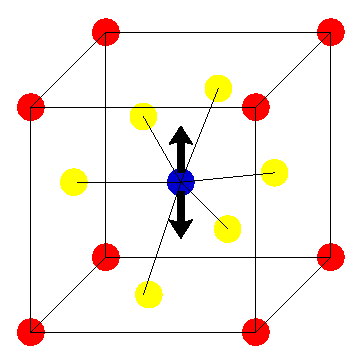
\includegraphics{FeRAM}
\caption{ FeRAM example.\label{fig:FeRAM}}
\end{figure}

\textcolor{blue}{
\paragraph{Polymer Memory:} this technology is based on polymer materials with special
formulation. This memory is non-volatile, non-destructive read, high
density, low on voltage and low on power consumption. Another
interesting feature of this kind of memory is its low cost. There is
no estimate to when this technology will be on the market, since it is
still a laboratory product.  
}

\textcolor{blue}{
\paragraph{PFRAM (Polymeric Ferroelectric Random Access Memory):} this memory 
store data by changing the polarization of polymer, which is between
metal lines. This is a non-volatile memory and has fast read and write
speed (initial read and write speed comparable to flash). The problem
with this technology is its destructive read. Intel~\cite{Intel:2003}
is one example of companies that are investing on this
technology~\cite{Magee:2002}.  
}


\chapter{Operating Systems and Flash Memory}

\emph{Flash memory} has been accepted as the industry ``de facto''
standard solution for non-volatile storage in embedded systems.
However, turning a "raw" flash memory chip into a usable
disk-replacement for embedded applications is a rather complex task.
This chapter discusses the use of flash memory in embedded systems from
the point of view of the operating system, including device drivers,
filesystems, and update support.


\section{Device Drivers}

Some flash memory gadgets include additional components that emulate
an ordinary hard disk to the operating system. Such devices are
usually interfaced to a filesystem through a traditional hard disk
device driver that knows nothing about the peculiarities of flash
memory operation.  Nevertheless, ordinary flash memory units, as used
in most systems, do not include such additional disk-emulation
logic. They rely on specially designed device drivers to interface
them to the file subsystem's disk-like interface.

A \emph{flash memory device driver} differs from a RAM-disk driver in
that, besides mapping volume blocks into memory pages, it must also care
for an efficient management of flash memory limitations like sector
lifetime (for erasing), intra-sector rewriting of data, etc. Some device
drivers will handle flash particularities internally, exporting a
disk-like interface that supports the installation of an ordinary file
system on a flash memory device. A second approach would be to export an
interface with some flash-specific services. This second approach could
probably lead to a more effective flash usage, but it would also require
a flash-specific filesystem. Therefore, most systems opt for flash
device drivers that emulate an ordinary disk.


\subsection{Flash-specific Tasks}

Independently of the strategy chosen to export services, a flash driver
must handle several flash-specific tasks. The most important are
summarized in this section.

Traditional filesystems are designed to update data in place. The same
disk sectors are constantly rewritten with new data.  This is a
reasonable mode of operation for magnetic media, but at odds with flash
memory, since there is a limitation in the number of times a flash can
be rewritten. Updating data in place on a flash would cause some sectors
(e.g. directories nodes) to expire their lifetimes far earlier than some
other sectors. Furthermore, today's typical flash sectors ($\sim$ 64
Kbytes) are too large to be directly mapped as disk blocks ($\sim$ 512
bytes).

There are two basic strategies to support the update of a small disk
block stored in a larger flash memory sector: erase-before-write and
remapping (not-in-place-update). The first strategy consists in coping
the whole sector to a temporary sector, erasing it, coping back
unaltered blocks, and writing the new contents of the block being
updated to the proper offset in the just-erased sector. The temporary
sector must be subsequently erased.  The second strategy consists in
having a translation table that maps logical disk blocks in physical
portions of flash sectors (\emph{frames}). In this way, updating a block
can be achieved by writing the data into a new frame and updating the
translation table.  Afterward, the old frame is marked ``dead for
posterior clean-up procedures.''

The remapping strategy has obvious performance advantages over immediate
rewriting. Besides, it allows for the homogeneous usage of sectors, so
the whole flash ages uniformly (\emph{wear-leveling}). However, it has
an important shortcoming: the need for \emph{garbage collection}.
Flagging frames as ``dead'' means leaving garbage behind in flash
sectors that must be later collected. Ideally, this operation would be
delayed until all frames in a sector are flagged ``dead'', so reclaiming
the sector (erasing it and putting it back at the free frame/sector
list) could be done without a single copy. In practice, however, it is
probable that many sectors will contain a mixture of dead and live
frames. In this case, live frames of a sector must be moved to other
sectors before its dead frames can be reclaimed.

Confronting remapping advantages (performance and wear-leveling) with
its disadvantages (garbage collection) usually leaves a positive result,
specially if the garbage collection procedure is implemented in such a
way that reclaiming is preventively performed in advance on flash's idle
time. Consequently, remapping became the most common approach to support
data update in flash memories.

Other flash-specific duties of device drivers are:

\begin{description}
  
\item[Data protection:] flash memory units often support write
  protecting individual sectors. This can be used to protect critical
  data such as bootstrap and operating system kernel.
  
\item[Fault recovery:] since most flash memory units do not implicitly
  validate write operations, a flash device driver must periodically
  check for data integrity.  If a failure is detected, the driver can
  mark the corresponding sector as ``bad'' and try to rewrite the data
  in other place. Write failures can be an indicative of life-time
  expiration.

\end{description}


\subsection{Case Studies}

At present time, there are many \emph{flash driver layers} available
both for commercial and open-source operating systems. The most
significant example of driver that supports windows-like filesystems is
the proprietary \emph{Flash Translation Layer}, while the \emph{Memory
  Technology Device} driver is mostly adopted by open-source systems.
 
\paragraph{Flash Translation Layer (FTL):}

FTL is a sector-based flash manager that provides logical to physical
sector mapping, thus enabling a flash to look like an ordinary disk to
the operating system~\cite{FTL:1998}. As a rule, FTL supports any ordinary
filesystem to be installed on a flash, but it is mostly deployed with
windows-like systems such as VFAT. In order to achieve this, FLT defines
small ``virtual blocks'' that are dynamically mapped into the flash
memory unit (not-in-place-update), thus granting wear-leveling.

As depicted in figure~\ref{fig:ftl}, FTL divides the flash into one or
more \emph{Erase Units} (EU). The size of an EU depends on the flash
sector size.  Each EU is divided in one \emph{Erase Unit Header} (EUH),
one \emph{Block Allocation Map} (BAM) and several \emph{Read/Write
  Blocks} (RWB). The EUH contains information about the Erase Unit such
as its size and the size of RWBs. The BAM keeps allocation information
about every RWB in the EU and is usually stored after EUH. It is
arranged in 4-byte entries, each describing the state of a RWB (deleted,
bad, free, or allocated).

Read/Write Blocks can store three different types of data: \emph{Virtual
  Block Data} (VBD), \emph{Virtual Block Map Pages} (VBM) and
\emph{Replacement Pages} (RP).  VBD is the user-data block exported to
the host filesystem. VBM contains information to perform address
translation. It is organized as a table of 4-byte entries, each one
pointing to the logical address on the flash where the corresponding VBD
resides. The virtual block number supplied by the host filesystem is
used as an index into this table.  RPs are hold recent updates to an
associated VBM, thus extending its live-time.

\begin{figure}[h]
\centering
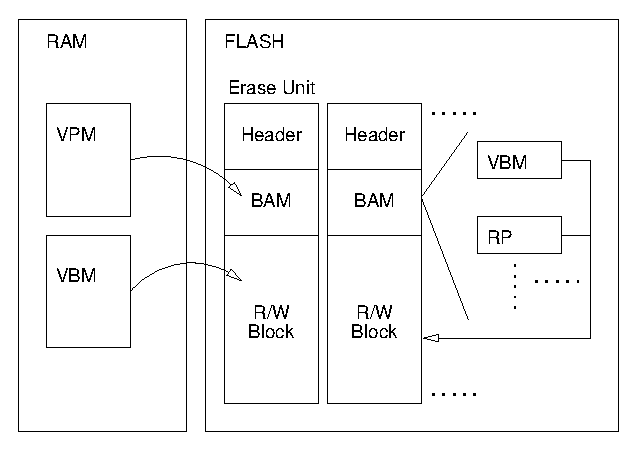
\includegraphics[scale=1.0]{ftl}
\caption{FTL architecture.\label{fig:ftl}}
\end{figure} 

During initialization, FTL scans the Erase Unit Header and the Block
Allocation Map of all Erase Units. Some flash sectors do not have an EUH
and are taken as \emph{spare blocks} or \emph{transfer units} that are
used on recovery/reclaim methods. Is not necessary to keep all the VBM
stored on flash. Users can choose between keeping VBM in RAM, in flash
or both of them. At initialization time, \emph{Virtual Page Maps} (VPM)
are created to hold the contents of those VMBs kept in flash (the same
happening to Replacement Pages).


\paragraph{Memory Technology Device (MTD):}

MTD drivers~\cite{MTD:2002} are a new class of drivers developed under
Linux specifically for the embedded system area. The main advantage of
MTD over conventional device drivers is that MTD drivers define a
generic Linux subsystem for memory devices, in particular flash
devices.  Besides exporting the typical \emph{raw block} interface for
disk emulation, MTD drivers also export a \emph{raw character}
interface that allows filesystems to access the flash as if it were
an ordinary linear memory device\footnote{The \emph{raw character}
interface is used by the Journaling Flash File System described later
in section~\ref{sec:fs}.}.

The main focus of the MTD project is to define a generic interface
between hardware drivers and the upper layers of the operating system.
In this way, hardware drivers need to know nothing about memory storage
issues such as wear-leveling and garbage collection, simply providing
routines for reading, writing and erasing. The MTD subsystem is divided
in two types of modules: ``users'' and ``drivers''. Drivers are the
modules which provide raw read/write/erase access to physical memory
devices.  Users are the modules which use MTD drivers providing a
higher-level interface to user-space.  MTD subsystem architecture is
depicted in figure \ref{fig:mtdarch}. 

\begin{figure}[h]
\centering
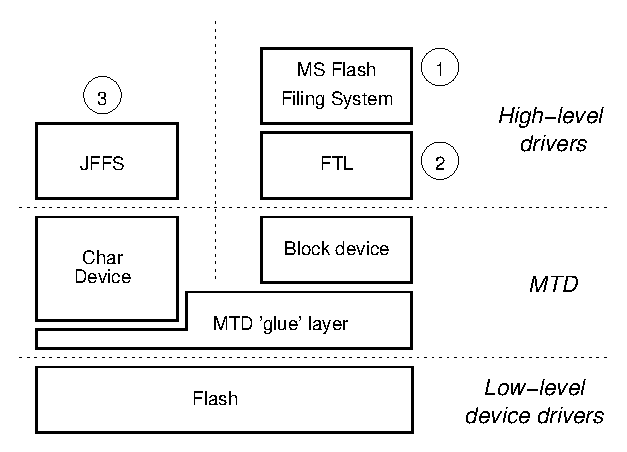
\includegraphics[scale=1.0]{mtdarch}
\caption{MTD Architecture.\label{fig:mtdarch}}
\end{figure} 


\textcolor{blue}{
\section{Future Device Driver Technology:}
}

\textcolor{blue}{
According to the literature studied, the future of flash memory device
drivers focus mainly on 2 ideas: (1) flexibility in the interaction
between hardware and the system; and (2) system (re)adaption with
existing and future management algorithms. Following this idea, HTD is
the closest to that. Its capability of readapting to different
algorithms and its flexibility in interacting with hardware and
filesystem is the challenge to this project. This section discusses
future drivers functionalities and its management.
}

\textcolor{blue}{
\paragraph{Hardware Mediator Technology (HMT):} HMT project consists 
of ``low level software pieces'' or ``low level components'' called
pseudo-drivers, implemented for hardware devices specifically for the
embedded system area. It has a ``generic software philosophy'' to
interact with different kinds of hardwares like processors, buses,
devices, controllers, etc. Hardware Mediators have been studied inside
Application Oriented Object System (AOOS)\cite{Froehlich:2001} context
by LISHA (Hardware and Software Integration Laboratory).
}

\textcolor{blue}{ Initially, the HMT project focused on hardware
mediator abstract elements for one hardware platform that would be
used by EPOS\cite{Froehlich:ooosw:1999} system abstractions and EPOS
scenario aspects\cite{Froehlich:sci:2000}. It was born principally to
solve hardware specific architectural dependencies that implies a
``layer overhead'' and a ``difficult software maintenance'', present
in other ``generic design technologies''. }

\textcolor{blue}{ However, these mediators are not intended to build a
``universal virtual machine'' for EPOS project, but hide the
peculiarities of some hardware components. HMT used this idea to build
a more efficient ``pseudo-driver'' layer specifically for RIFFS
(showed later).}

\textcolor{blue}{ HMT, in its flash project context, differs from
traditional drivers because they are compiled with an application (it
means that HMT is just some code from an application point of view)
but gives the idea of a driver layer for the software architecture
designer. \footnote{ HMT just exists in source code and it is never
found ``compiled alone''.} }

\textcolor{blue}{ The aim of this ``pseudo-driver'' layer is similar
to MTD (Memory Technology Device) where \emph{hardware access layer}
needs to known just basic operations like read, write and erase,
ignoring the (complex) media management algorithms. The difference
between these two technologies is the fact that HMT is not a
``compiled-layer'' to interact with hardware and filesystems.  }

\textcolor{blue}{ As mentioned before, HMT is a group of
components. Each HMT component implements one generic interface
(read/write/erase, exported to file system) to interact with a
specific piece of hardware, and its architecture is showed in figure
\ref{fig:hmtarch}.  }

\begin{figure}[h]
\centering
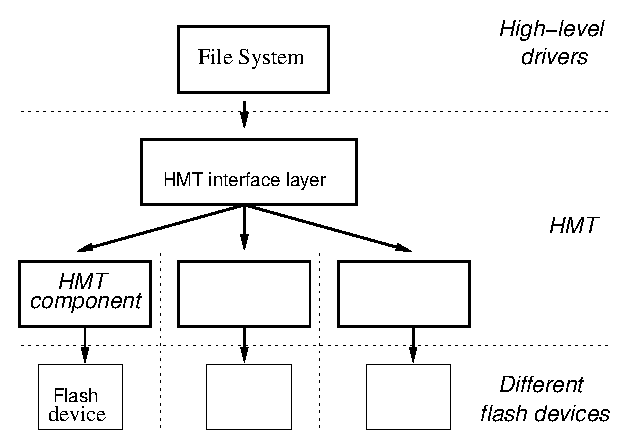
\includegraphics[scale=1.0]{hmtarch}
\caption{HMT Architecture.\label{fig:hmtarch}}
\end{figure} 

\textcolor{blue}{ When a filesystem needs to interact with the
hardware, it does it via HMT, thus promoting the idea of transparent
portability.  Each hardware mediator itself is not portable, just its
idea; they are specifically designed and implemented for each
plataform in an easy way (provided by its conception and its software
engineer).  }

\textcolor{blue}{ As mentioned before, mediators are themselves
hardware dependent, being sometimes coded in assembly, using macros,
or static metaprogramming techniques. Because HMT is compiled with its
up-layers, different file systems will exists for each kind of flash
memory, increasing performance compared to ``generic software
implementations'', because it doesn't need to execute unnecessary
code.  }

\section{File Systems\label{sec:fs}}

Application programs are able to store and retrieve data from flash
memory units through the services of a device driver. Very often,
however, the approach of directly controlling the storage of data
becomes inadequate, even in embedded system. If different applications
are to autonomously store data on the same flash memory, or if stored
data is intensively manipulated, then installing a \emph{filesystem}
will usually be a more effective approach.

Although the filesystem scene is a very rich one, few filesystems have
being proposed for flash memory. This is mainly due to the fact that
most flash device drivers realize a disk-like interface that enables the
installation of non-flash-specific filesystems on top of flash memory
units.  Nevertheless, a flash-specific filesystem will probably be
advantageous in regard to a disk filesystem, since it has the
opportunity to directly handle the limitations imposed by the
technology.


\subsection{Case Studies}

\paragraph{True Flash File System (TrueFFS):}

M-Systems' TrueFFS~\cite{TrueFFS:2002} implements itself patented
standard called FTL, and exports the flash memory as a hard disk drive
to the operating system. The FTL itself (implemented as a TrueFFS's
module) automatically handles wear-leveling, data protection, sector
mapping, garbage collection, and fault recovery. Though called a file
system, from a more strict point of view, TrueFFS would be considered
a flash device driver.  Indeed, TrueFFS requires the DOS
FAT\footnote{DOS FAT is supported for all block devices} filesystem
on top of it, and Figure \ref{fig:trueffs} shows an example of how
TrueFFS interacts with filesystem, operation system and FTL
module. TrueFFS encapsulates the FTL module and then, exports block
device services to filesystem and implements specific operation
system integration.

\begin{figure}[h]
\centering 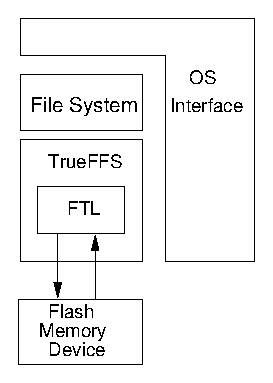
\includegraphics[scale=1.0]{trueffs}
\caption{TrueFFS Layer inside Operate System
context.\label{fig:trueffs}}
\end{figure}


\paragraph{Journalling Flash File System (JFFS):}

Axis Communications' JFFS~\cite{JFFS:2002} differs from the traditional
``virtual disk'' approach (used by TrueFFS for example) while
implementing a flash-specific filesystem for embedded systems. JFFS
version one (JFFS1) is a purely log-structured file
system~\cite{Rosenblum:1992} and its improvement in version
two~\cite{Woodhouse:2001} (JFFS2) includes compression and more
efficient garbage collection.

The version one of JFFS (JFFS1), has two kind of structures: the (1)
\emph{node} structure (kept in flash device) called struct
\emph{jffs\_raw\_inode}; and the (2)\emph{inode} struct (kept in RAM)
is the struct as each node is associated. The inode header contains
``the inode number'', ``the inode data'' and all ``metadata'' related with it
(like the name of the inode and the parent's inode number).Each node
is associated with a version (hold in header) higher than all previous
nodes belonging to the same inode number. This schematic is used by
the host filesystem to know if the node is actually deleted. Also,
there is a restriction on the maximum size of physical nodes, so large
files will have many nodes\footnote{Because symbolic links and
especially device nodes, have small amounts of data, the data are not
fragmented into many different nodes on the flash} associated with
them.

JFFS1 has 3 main disadvantages: (1) compression is not supported; (2)
hard links are also not supported; (3) inefficient garbage collection
(because erase method get the first flash block in the log, without
any criteria). An garbage collection inefficiency example is explained
when the system contain a considerable amount of static
data~\footnote{Static Data could be interpreted as libraries and
executable files}: Suppose a system with 12MB of static data. In this
system the garbage collection could move all of this static data.

The second version of JFFS (JFFS2) improves the disadvantages caused by
JFFS1 and its code was intended to be portable, in particular to eCos,
Red Hat's embedded operation system~\cite{ECOS:2002}. While the original
JFFS had only one kind of node, JFFS2 is more flexible~\footnote{This
flexibility is compared as traditional UNIX-like filesystems on each
inode is a distinct entity from directory entries}, allowing 3 types
of nodes: (1) the \emph{jffs2\_nodetype\_inode} is most similar to the
struct \emph{jffs\_raw\_inode} from version 1. It contains all the
inode metadata as well as the range of data belonging to the
inode. However, it no contains a file name nor the number of the
parent inode. One important observation in this version 2 (as
traditional UNIX-like filesystem), an inode is removed when the last
directory entry referring to it has been unlinked, and there is no
open file descriptors; (2) the \emph{jffs2\_nodetype\_dirent}
represents a directory entry, or a link to an inode. A link is removed
by writing a dirent node with the same name but with target inode
number zero - and obviously a higher version. With this difference
between inodes and directory entries, the JFFS2 could support hard
links; (3) the \emph{jffs2\_nodetype\_cleanmarker} is written to a
newly erased block to show that the erase operation has completed
successfully and the block may safely be used for storage. This node
type was introduced after JFFS2 had started to be used in real
applications to avoid the problems of extensive power fail (because if
power is lost during an erase operation, some bits in the medium may
be left in an unstable state).

The second and third challenge in JFFS2 was its ``data compression''
and its ``garbage collection improvement'' respectively. Two
compression algorithms were developed for use in JFFS2, and also the
JFFS2 code can contain yet another copy of the \emph{zlib compression
library} which is present in the Linux Kernel source.  Because the new
garbage collection algorithm, the high-level layout of JFFS2 also
changed from a single circular log format to an better performance
decision collector format.  This new format work with increased
efficiency by collecting from one block at a time and making decisions
about which block to garbage collect from next. To help garbage
collection JFFS2 code also keeps a number of linked lists of
structures representing individual erase blocks. 

The majority of erase
blocks will be on the \emph{clean\_list} or the \emph{dirty\_list},
which represent blocks full of valid nodes and blocks which contain at
least one obsoleted node, respectively. In a new filesystem, many
erase blocks may be on the \emph{free\_list}, and will contain only
one valid node (a jffs2\_nodetype\_cleanmarker).  

The operation of JFFS2 is very similar to that of the original JFFS
where nodes, albeit now of various types, are written out sequentially
until a block is filled, at which point a new block is taken from the
\emph{free\_list} and writing continues from the beginning of the new
block.  Different of that three lists (clean\_list, dirty\_list and
free\_list) JFFS2 also keep in RAM a full map of filesystem. This map
is constructed in mounting (by scanning the entire flash) and is
supported by 2 structures: (1) \emph{jffs2\_inode\_cache} and (2)
\emph{jffs2\_raw\_node\_ref}. For each inode on the flash, there is a
struct \emph{jffs2\_inode\_cache} showed in figure \ref{fig:jffs2}
which stores its inode number, the number of current links to the
inode, and a pointer to the start of a linked list of the physical
nodes which belong to that inode\footnote{It is important to note that
an inode is build by a linked list of nodes.}. Each physical node on
the medium is represented by a smaller struct
\emph{jffs2\_raw\_node\_ref}, also show in figure \ref{fig:jffs2},
which contains two pointers to other raw node references, the physical
offset and total length of the node.

\begin{figure}[h]
\centering
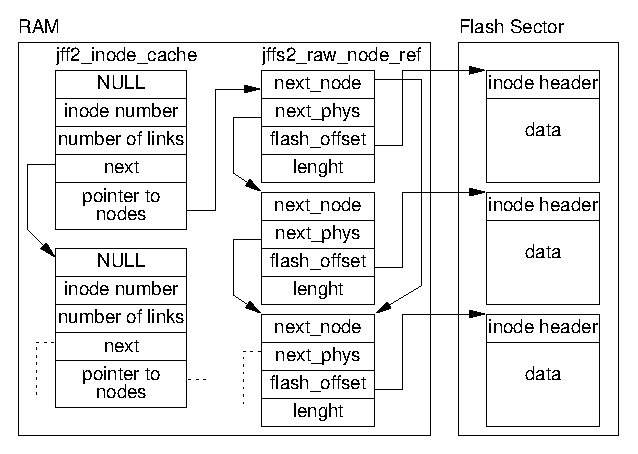
\includegraphics[scale=1.0]{jffs2}
\caption{JFFS2 Architecture.\label{fig:jffs2}}
\end{figure} 


Mounting a JFFS2 filesystem involves a four-stage operation. (1) the
physical medium is scanned and the \emph{jffs2\_inode\_cache} are
allocated and inserted into the hash table for each inode for which
valid inodes are found and the \emph{jffs\_raw\_node\_ref} either; (2)
a first pass through all the physical nodes is made, obsoleted nodes
can be detected and the ``number of links field'' is increased for
each valid directory entry node; (3) a second pass is then made to
find inodes which have no remaining links on the filesystem and
delete them. (4) a third pass is made to free the temporary
information.


\paragraph{Embedded File System (Efsys):}

\emph{QNX Software Systems} Efsys~\cite{QNX:2002} combines the functions of
a filesystem manager and a device driver to manage a Flash filesystem
om memory-based media. Because Efsys includes the device driver for
controlling the hardware, there are separate versions of Efsys for
different flash manufacturer. Each logical driver is called a
\emph{socket}, which consists of a contiguous an homogeneous region of
flash memory. Each socket may be divided into one or more
\emph{partitions}.  Actually there are two types of partitions
supported: \emph{raw partitions} and \emph{flash filesystem
partitions}. A raw partition is any partition that doesn't contain a
flash filesystem and may contain an image filesystem or some
application-specific data. A flash filesystem partition exports the
\emph{POSIX-like} filesystem, which uses a QNX proprietary format to
store data on the flash devices. This format stores files and
directories as a direct linked list of \emph{extents}. QNX defines
\emph{extent} like one consecutive region on one media (flash, disk,
etc).  Normally one file have multiples \emph{extents}.  Through
literature studied, QNX flash filesystem supports the standard
\emph{POSIX} functionality like symbolic links, long filenames, etc;
but there are one exception: it doesn't support "hard links".  QNX
flash filesystem supports transparently data decompression from
flash. It is not true by compression ability, where the application
need explicitly call a function to do that.  When the flash is
formated by Efsys, the filesystem manager lock one (or more)
untouchable block called \emph{spare block}. This \emph{spare block}
will be used by garbage collection when system reclaim space. The QNX
flash filesystem also has the expected features for flash filesystems
like wear-leveling and fault recovery.

\paragraph{Other technologies:}
\begin{itemize}
   \item Virtual File System (VFS): PalmOS' VFS~\cite{VFS:2002}
     requires the flash memory unit to be encapsulated in a device
     that emulates an ordinary storage device and therefore cannot be
     considered a flash filesystem. Nevertheless, it implements a
     sort of lightweight database system that may be of interest to
     some embedded applications.  VFS stores both programs and data as
     collections of records that can be accessed via a database
     interface: a rather convenient approach for \emph{Personal
     Information Manager}~[PIM] applications.
  \item Microsoft Flash File System (MFFS): Microsoft's MFFS is a
     substratum for DOS FAT filesystems.  Similarly to the TrueFFS,
     it handles all traditional flash tasks. One of its peculiarities
     is the adoption of variable size block, which can optimizes
     garbage collection: a large segment of garbage in a block can be
     converted into a new garbage-only block for immediate reuse.
\end{itemize}


\textcolor{blue}{
\section{Future File System Technology:}
}

\textcolor{blue}{ Since the beginning of flash filesystems, many
algorithms have been suggested to overcome flash deficiencies. This
section emphasizes on the last studies in flash management, that will
become the next generation of this technology in a near future. Inside
this new generation there is the management of index structures as
showed in RIFFS and B-Tree Layer for Flash.  }

\textcolor{blue}{
\paragraph{Reverse-Indirect Flash File System (RIFFS):} \emph{Research Group 
of Hardware and Software Integration Laboratory} (LISHA) has been
studying a different manner to store data in (specifically) flash
memories. The aim of the flash filesystem research project is to
develop a complete flash filesystem totally flexible and customizable
(generic in other words), but without compromising performance. To
meet this expectation the group uses two non-usual ideas: (1) the
rescue of the old paradigm \emph{variable data-block length} and, (2)
\emph{reverse linked-list and indirect-tree management}, to compensate
for flash memory disadvantages.
}

\textcolor{blue}{ The purpose of RIFFS is not to develop a new garbage
collection, nor a new wear leveling algorithm but implement a new way
to store data in flash memories and try to group all the efficient
flash management algorithms (or at least most of them) in an easy way
and without overhead. Its structure is like a linked-list but
indirect. In this manner, the filesystem tree appears in a reverse
form, and this is the reason for its name. The RIFFS architecture is
showed in figure \ref{fig:riffs}.  }

\begin{figure}[h]
\centering
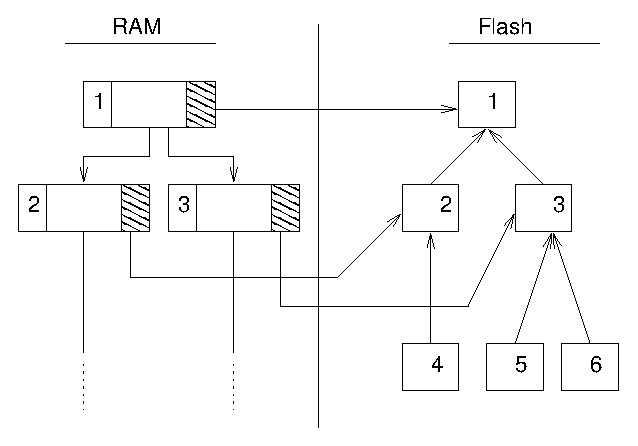
\includegraphics[scale=1.0]{riffs}
\caption{RIFFS Architecture.\label{fig:riffs}}
\end{figure} 

\textcolor{blue}{ With the reverse tree, RIFFS eliminates some aspects
in garbage collection (like inside-block dirty pointers or logical to
physical map), and \emph{variable data-block length} improves wear
leveling. To do its ``job'', there are two main data-structures: (1)
reverse\_node, present in media, and (2) mounted\_map\_node, present
in RAM memory, as shown in figure \ref{fig:riffs}.  }


\textcolor{blue}{ A reverse\_node just carries a logic number, its data
and a pointer to a parent-node. On mounting, the entire flash is
scanned and a direct-tree is built in RAM memory.}


\textcolor{blue}{ \paragraph{B-Tree Flash Translation Layer (BFTL):} Research Group 
of Computer Science Department of National Taiwan University proposed
``An Efficient B-Tree Layer for Flash-Memory Storage
Systems''~\cite{Btree:2002}. }

\textcolor{blue}{ For index structures (as B-Tree structures) which
require major modifications, block-oriented access over flash memory
could introduce a significant number of redundant writes (with data
and pointers management, required by B-tree). This project proposes
the efficient management of B-Tree index access over flash memory.  }

\textcolor{blue}{ The focus of this project is on an integration of
B-Tree index structures and the block-device emulation mechanism
provided by FTL (Flash Translation Layer), resulting on an insertable
module called BFTL. BFTL sits between the application layer and the
block-device emulated by FTL. The BFTL module is dedicated to those
applications which use services provided by B-Tree indexes. B-Tree
index services requested by the upper-level applications are handled
and translated by BFTL, and then block-device requests are sent from
BFTL to FTL.  }

\textcolor{blue}{ B-Tree node is physically represented by a
collection of index units, and to help BFTL to identify the index
units of the same B-Tree node, a \emph{node translation table}(NTTab)
is adopted. NTTab is introduced as an auxiliary data structure to
collect index units efficiently. Basically, the \emph{node translation
table} maps a B-Tree node to a collection of index units supplied by
FTL, and this index units could come from different sectors on
flash. The \emph{node translation table} is shown in
Figure~\ref{fig:Btree}.  }

\begin{figure}[h]
\centering
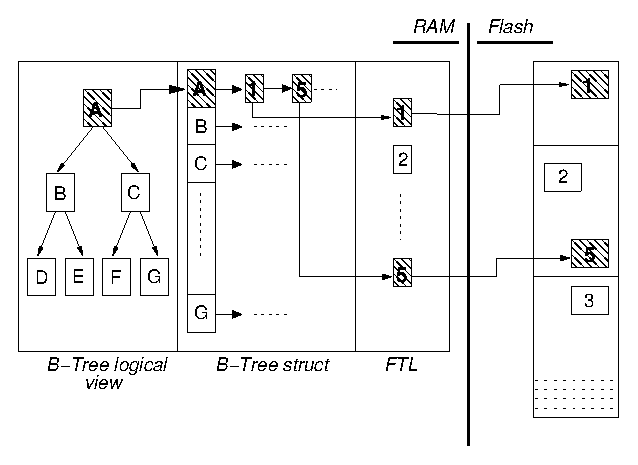
\includegraphics[scale=1.0]{btree}
\caption{B-Tree node translation table.\label{fig:Btree}}
\end{figure} 

\textcolor{blue}{ BFTL is constantly built in RAM memory, according to
its node access.  When a B-Tree node is visited, all the index units
belonging to the visited node is collected and the NTTab could grow
unexpectedly.  To solve this problem researches propose to compact the
\emph{node translation layer}, and a variable (defined by user) is
used to control the maximum length of the lists. After that, the
compacted NTTab is written back to flash memory. This operation
introduces an overhead in system, and obviously, the ``system
engineer'' must choose between the compaction (in other words: the
length of list) and the performance.  }

\section{Update Support}

An apparently unimportant aspect of operating systems designed to
operate from/on flash memories is the way they can be updated, for the
time in which embedded systems were delivered with absolute, immutable
firmware is long gone. Today's embedded systems must consider regular
upgrade operations for firmware, operating system, and applications
--- the popular ``system re-flashing''.

One aspect in which the operating system can easy or difficult updating
concerns the way it is stored in flash. If the system is a monolithic
piece of software installed on a predefined location in flash, it is
very likely the upgrading it will require the whole flash to be erased,
since the installation of a larger system image could corrupt
preexisting filesystem structures. Moreover, some systems are directly
executed from flash and allow applications to make absolute references
to internal functions. In this case, updating the system implies in
updating all applications. Such a condition could have serious
consequences for perpetual applications that store context information
in the flash.  For an example consider an \emph{odometer} application on
a car: re-flashing the system without preserving the current mileage
count would transform an old chariot in a ``0 Km''. Typical Windows CE
installations present such shortcomings.

Re-flashing side-effects can be avoided, or at least minimized, if the
operating system is itself installed in the filesystem. In this case,
upgrading the operating system solely requires some files to be
overwritten/added and has no direct effect on applications. Typical
Linux distributions for embedded systems function in this way. In
particular, the different Linux distribution provides a tool called
``apt-get'' that is able to download packages from the network (via
``wget'') and install/upgrade them in a consistent way. Indeed, embedded
Linux distributions usually inherit on-the-fly kernel upgrade mechanism from
desktop distributions called \emph{loadable kernel} modules.

\subsection{Case Studies}
WindowsCE uses the first approach so it have to rewrite the entire
data in the memory.
Pocket Linux otherwise uses the second approach and can even change
kernel on-fly, updating just the selected modules (files).

\paragraph{WindowsCE for Automotive Update}

The current version of Windows CE does not include the necessary API
to update all or part of the Flash. Fortunately, it was done by a
small Operating System called \emph{burnos}~\cite{Burnos:2002} (just in
Automotive WindowsCE version~\cite{Wincefa:2002}).

Burnos is a temporary second operating system that executes while the
current OS is being reprogrammed. Because burnos reside in the same
block as the boot code, if the update process is interrupted, the
utility must be available to resume or redo the update. On power-up or
reset, if the boot loader does not find a valid image in the rest of
the Flash, it will invoke the update OS to install the program.

The WindowsCE operating system and applications are a single binary
image, so they are written sequentially into the rest of the Flash
without regard for block boundaries.  To update the OS and the
applications, The burnos performs some tasks showed on
figure~\ref{fig:winupdate}: (1) Take control of the system. Since
Windows CE does not implement this capability or support a partial
update, the utility must preempt the operating system; (2) Erase all
blocks that do not contain boot code. The entire binary image must be
erased and reprogrammed; (3) Input the new binary image. All code
necessary to receive the new program must be included in the utility,
because the rest of the code will have been erased; and (4) Program
the new image into the Flash.

\begin{figure}[h]
\centering
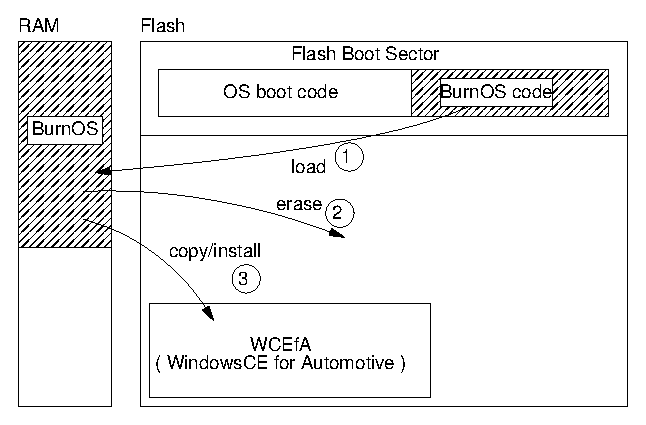
\includegraphics[scale=1.0]{winupdate}
\caption{WCEfA update schematic.\label{fig:winupdate}}
\end{figure} 

During the 1st. phase, the system reboots 2 times. The initial boot
happen just to clear RAM. Next, the system loads the burnos, and modify
the system loader to boot burnos. The last 3 phases, there are three
reboots: the first reboot happens to copy Burnos to RAM and then, it
sets a special boot-mode and boots again. Next, the temporary OS
started a configuration routine. Last, the update process loads the
new image into RAM. Once loaded and verified, the flashing
begins. After the flashing has completed, the boot-mode returns to
original configuration and upon final reboot, the system comes up
under the new version.


\paragraph{Linux Update support}

The most basic way to add functions (routines) in Linux Kernel is to
put code inside it. But if there is necessity to divide it in distinct
peaces (called modules), you can also add code by Loadable Kernel
Module (usually called LKM) ~\cite{LKM:2002}. 

LKMs are attached to Linux Kernel dynamically by loading modules that
implement protocol handlers, where these modules install function
pointers into a protocol handler list. The LKM is divided in four kind
of modules: (1) device drivers (used to communicate with a piece of
hardware); (2) filesystem drivers (used to interprets the contents of
a filesystem as files and directories); (3) system calls (used to get
services from kernel) and (4) executable interpreters (used when an OS
has more than one kind of executable files). The kernel isolates
certain functions, including these, especially well so they don't have
to be intricately wired into the rest of the kernel. 

The most advantage, in updating context, is that LKM helps the system
to update just modules, not the entire Kernel code, and this saves
time to rebuild (recompiling) and installing it.  The ``module's
load'' can be done in three different ways: (1) automatically, using
scripts; (2) manually from the command line (not usual in embedded
systems); or (3) loaded directly from kernel as need (like devices
drivers for example), normally done in kernel boot. Linux uses itself
tools to do this ``job'', called modutils. Modutils is a package that
has some commands to handle the modules (like load\_module,
unload\_module, verify\_module, etc).

An LKM lives in a single ELF object file, normally named like
"file.o". The "file.o" dependencies are resolved in load-time
(dynamically). Although advantages of LKM, is common to find in
embedded systems all the module's code inside the kernel because its
better performance~\footnote{The balance between performance and
flexibility can be defined by Software Architecture Engineer based in
its knowledge.}. The figure \ref{fig:lkm} shows an example of how some
library could be updated via LKM without recompiling/installing the
entire system.

In phase one the (1)``lib.o'' and (2)``startup\_configuration'' are
erased; (3)``loaded\_lib.o'' is unloaded and (4)``kernel reference''
is destructed. The second phase the (5)``new\_lib.o'' and
(6)``new\_startup\_configuration'' are record
(7)``new\_loaded\_lib.o'' is loaded and (8)``new kernel reference''
are build. This update method is done without reboot the system. This
method could vary for each Linux distribution.

\begin{figure}[h]
\centering 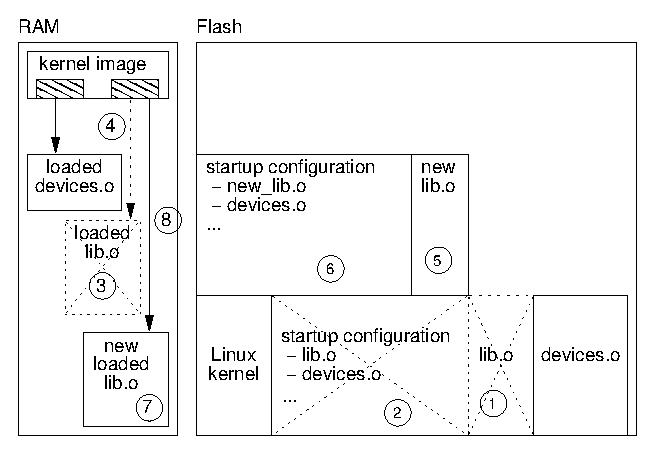
\includegraphics[scale=1.0]{lkm}
\caption{WCEfA update schematic.\label{fig:lkm}}
\end{figure}

In update context, there is also one important tool (or package) to do
the system update and its name is ``apt-get''. Apt-Get is a package
management system that is designed on debian linux systems and ported
to another distributions. It has the ability to connect to a server
``repository'' (on internet and/or locally) and checks (automatically)
all ``package dependencies'' required. Because apt-get is implemented
in GPL~\footnote{General Public License (GPL) is intended to guarantee
your freedom to share and change free software--to make sure the
software is free for all its users.}~\cite{GPL:2002} designers/programmers
has the advantage to (re)adapt this software to its
necessities. Apparently all the linux distributions has this capability
to update dynamically modules and packages either in embedded systems.

\bibliography{flash}


\end{document}

